\chapter{Εισαγωγή} \label{Chapter1}


%----------------------------------------------------------------------------------------
%	SECTION 1
%----------------------------------------------------------------------------------------

\section{Συστήματα Διμερούς Τηλεχειρισμού} \label{Chapter1Section1}
Τα \textbf{Συστήματα Διμερούς Τηλεχειρισμού Ηγέτη-Ακόλουθου - ΣΔΤΗΑ} (Leader-Follower teleoperation systems) είναι συστήματα κλειστού βρόχου που αποτελούνται από δύο ρομποτικούς βραχίονες: τον ηγέτη (Leader), ο οποίος χειρίζεται από έναν άνθρωπο, και τον ακολούθο (Follower), ο οποίος έχει ως κύριο στόχο να ακολουθεί και να αναπαράγει με ακρίβεια την τροχιά του πρώτου. Η γενική τους μορφή παρουσιάζεται στο Σχήμα (\bref{generic_implementation}).

\bigskip
Με τη ραγδαία ανάπτυξη που έχει σημειωθεί στον χώρο της ρομποτικής, τα συστήματα αυτά έχουν αποκτήσει ιδιαίτερη σημασία, καθώς προσφέρουν τη δυνατότητα εκτέλεσης σύνθετων και επικίνδυνων εργασιών σε απομακρυσμένα ή δυσπρόσιτα περιβάλλοντα, συνδυάζοντας την ανθρώπινη εμπειρία και κρίση με την ακρίβεια και την αντοχή των ρομποτικών συστημάτων, με απότοκο την μεγιστοποίηση της αποδοτικότητας και της ασφάλειας. Επιπλέον, σε τέτοιου είδους πρακτικές εφαρμογές, κρίνεται σημαντική η χρήση διμερούς επικοινωνίας, δηλαδή της παροχής απτικής ανάδρασης στον χειριστή. Αυτή η προσέγγιση τού προσδίδει διαδραστικότητα, με το να αισθάνεται δυνάμεις και αντιστάσεις που αντιμετωπίζει ο Ακόλουθος, βελτιώνοντας έτσι τον έλεγχο . 

\bigskip
Ως απόρροια των παραπάνω, σε συνδυασμό με την ταχεία πρόοδο και χρήση του διαδικτύου, των τεχνολογιών ασύρματης επικοινωνίας και κυρίως των ρομποτικών βραχιόνων, τα ΣΔΤΗΑ ενσωματώνονται σε ένα ευρύ φάσμα εφαρμογών. Συγκεκριμένα, εφαρμόζονται σε αποστολές έρευνας και διάσωσης με τη συγχρονισμένη τηλεχειριστική λειτουργία μεταξύ πολλών ρομποτικών συστημάτων, όπως προτείνουν οι Qureshi \textit{et al.} (2016)\cite{qureshi2016leader}. Επίσης, σε στρατιωτικά συστήματα επιτήρησης μέσω του τηλεχειρισμού στόλου UAV (Unmanned Aerial Vehicles) σε πραγματικό χρόνο, όπως αναφέρουν οι Hunukumbure \textit{et al.} (2013)\cite{hunukumbure2013teleoperation}, και στη ρομποτική χειρουργική, όπου ο χειρουργός-χειριστής ελέγχει το κύριο ρομπότ ενώ ένα ή περισσότερα ακόλουθα ρομπότ συντονίζουν τις ενέργειές τους, σύμφωνα με τους Guo \textit{et al.} (2018)\cite{guo2018leader}. Επιπλέον, τα ΣΔΤΗΑ χρησιμοποιούνται στην τηλεχειριστική λειτουργία αυτόνομων οχημάτων σε δυναμικά περιβάλλοντα, επιτρέποντας τη δημιουργία φάλαγγας οχημάτων υπό απομακρυσμένο έλεγχο, όπως παρουσιάζουν οι Jaloudi και Alloghani (2019)\cite{jaloudi2019leader}. Στον τομέα των υποβρύχιων ερευνών, αυτά τα συστήματα εφαρμόζονται σε επιθεωρήσεις αγωγών και εξερευνήσεις βαθέων υδάτων, όπως περιγράφουν οι Yuan \textit{et al.} (2021)\cite{yuan2021leader}. Στην αγροτική βιομηχανία, τα ΣΔΤΗΑ ενισχύουν την παραγωγικότητα σε εκτεταμένες γεωργικές εκτάσεις, όπου ένας ηγέτης-ρομπότ κατευθύνει πολλαπλές αυτόνομες μηχανές, σύμφωνα με τους Hou \textit{et al.} (2017)\cite{hou2017leader}. Τέλος, στη βιομηχανική παραγωγή, χρησιμοποιούνται για τον συντονισμό εργασιών σε επαναλαμβανόμενες ή επικίνδυνες διαδικασίες, όπως αναφέρουν οι Nakamura \textit{et al.} (2017)\cite{nakamura2017leader}.

\bigskip
Τα τελευταία χρόνια, το πρόβλημα του διμερούς τηλεχειρισμού Ηγέτη-Ακόλουθου με καθυστερήσεις επικοινωνίας έχει προσελκύσει σημαντικό ενδιαφέρον, και έχουν σημειωθεί αξιοσημείωτες πρόοδοι. Συγκεκριμένα, η ασυμπτωτική ευστάθεια του σφάλματος παρακολούθησης εξόδου έχει εδραιωθεί στα έργα των Chopra \textit{et al.} (2008)\cite{chopra2008synchronization}, Mohammadi \textit{et al.} (2012)\cite{mohammadi2012control}, Wang (2021)\cite{wang2021bilateral}, Estrada \textit{et al.} (2021)\cite{estrada2021stable} και Zhang \textit{et al.} (2022)\cite{zhang2022adaptive}. Επιπλέον, η ομοιόμορφη τελική φραγμένη συμπεριφορά έχει μελετηθεί στα έργα των Ohkawa και Yamashita (2011)\cite{ohkawa2011passivity}, Liu και Chopra (2013)\cite{liu2013control} και Abdessameud \textit{et al.} (2017)\cite{abdessameud2017leader}. Τέλος, η παθητικότητα του κλειστού βρόχου συστήματος μαζί με την ασυμπτωτική ευστάθεια του σφάλματος παρακολούθησης ηγέτη-Ακόλουθου έχει αναδειχθεί στα έργα των Forouzantabar \textit{et al.} (2012)\cite{forouzantabar2012bilateral}, Yan \textit{et al.} (2014)\cite{yan2014consensus}, Li και Kawashima (2016)\cite{li2016bilateral}, Nuño \textit{et al.}(2018)\cite{nuno2018control} και Su \textit{et al.}(2020)\cite{su2020bilateral}. Όμως, δεν προσφέρουν κάποια θεωρητική απόδειξη του ακριβές σφάλματος παρακολούθησης	πέρα από την ευστάθεια και την ασυμπτωτική του σύγκλιση, ένα πρόβλημα που επίλυσε το έργο (Bikas, Rovithakis) \textit{et al.}(2023)\cite{BIKAS20239972}. Το έργο αυτό, ακολουθώντας τον Έλεγχο Προδιαγεγραμμένης Απόκρισης (βλέπε \bref{Chapter2Section1}), καθώς και την ΕΠΑ λύση στο πρόβλημα παρακολούθησης μιας φραγμένης τροχιάς αναφοράς παρουσία χρονικών καθυστερήσεων στις καταστάσεις ή/και στην είσοδο ελέγχου (Bikas, Rovithakis) \textit{et al.}(2019) \cite{bikas2019enhancing}, \textit{et al.}(2021) \cite{bikas2021prescribed}, κατάφερε την ζητούμενη αξιόπιστη και προδιαγεγραμμένη παρακολούθηση με συγκεκριμένο ρυθμό σύγκλισης, θεωρώντας γνωστή και σταθερή καθυστέρηση στο κανάλι επικοινωνίας.

\bigskip
\begin{figure}[!ht]
  \begin{center}
    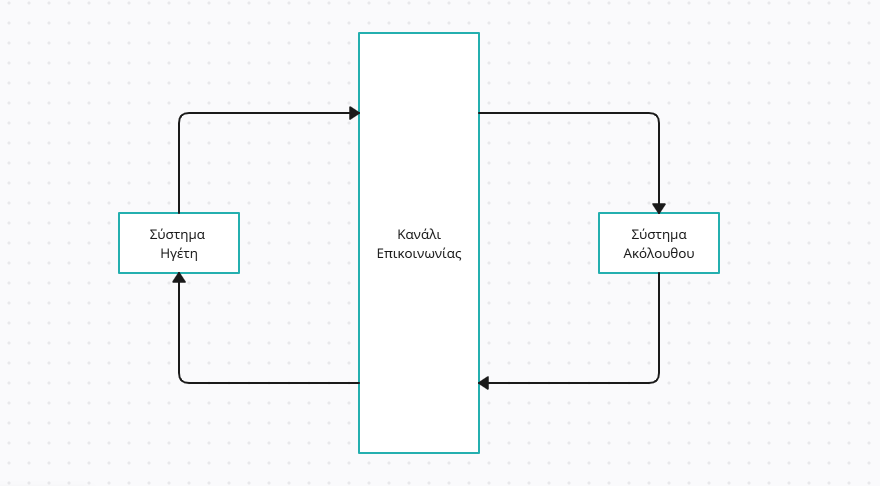
\includegraphics[width=1\linewidth]{Chapters/Chapter1/Figures/Generic_Implementation.png}
    \caption[Γενική Δομή των ΣΔΤΗΑ]{Γενική Δομή των ΣΔΤΗΑ}
    \label{generic_implementation}
  \end{center}
\end{figure}

\bigskip
Ένα σημαντικό ζήτημα που ανακύπτει είναι ότι οι καθυστερήσεις στο ψηφιακό κανάλι επικοινωνίας παραμένουν, στις περισσότερες περιπτώσεις, απρόβλεπτες και μη σταθερές, γεγονός που καθιστά τον έλεγχο σχεδιασμού της \cite{BIKAS20239972} αυτόν καθ' αυτόν ανεπαρκή να εγγυηθεί την ακριβή παρακολούθηση και την ευστάθεια του συστήματος. Οι καθυστερήσεις αυτές επηρεάζονται από παράγοντες όπως η ποιότητα του δικτύου, η απόσταση και οι συνθήκες λειτουργίας, δημιουργώντας σοβαρά προβλήματα στον συγχρονισμό μεταξύ Ηγέτη και Ακόλουθου, με αποτέλεσμα να υποβαθμίζεται η συνολική απόδοση και η ασφάλεια του συστήματος. Επιπρόσθετα, η μονομερής εστίαση στο πρόβλημα του τηλεχειρισμού του Ακόλουθου από τον Ηγέτη παραβλέπει την πιθανότητα ο Ηγέτης να οδηγήσει τον Ακόλουθο σε επαφή με εμπόδιο, χωρίς να το γνωρίζει ο χειριστής. Αυτή η κατάσταση μπορεί να προκύψει καθώς ο Ακόλουθος ελέγχεται με τρόπο ώστε να αναπαριστά πιστά την τροχιά του Ηγέτη, γεγονός που μπορεί να αποβεί καταστροφικό όταν δεν υπάρχει έγκαιρη ανατροφοδότηση ή όταν ο χειριστής δεν έχει πλήρη εποπτεία του περιβάλλοντος. Αυτά τα δύο βαρυσήμαντα και αντικρουόμενα προβλήματα – η έλλειψη σταθερότητας στην επικοινωνία και η αδυναμία πρόληψης συγκρούσεων – προκύπτουν οργανικά ως συνέπειες των προηγούμενων προσπαθειών.


%----------------------------------------------------------------------------------------
%	SECTION 2
%----------------------------------------------------------------------------------------

\section{Έλεγχος Προδιαγεγραμμένης Απόκρισης} \label{Chapter1Section2}
Οι προτεινόμενοι ελεγκτές σε αυτή την εργασία βασίζονται στην μεθοδολογία του \textbf{Ελέγχου Προδιαγεγραμμένης Απόκρισης-ΕΤΑ}(Prescribed Performance Control - PPC), η οποία προτάθηκε για πρώτη φορά στην \cite{bechlioulis2008robust}. Πρόκειται για μία μέθοδο, η οποία εγγυάται την προδιαγεγραμμένη απόκριση στο σφάλμα παρακολούθησης εξόδου επιβάλλοντας την σύγκλιση του σε μια προκαθορισμένη περιοχή γύρω από το μηδέν, με ρυθμό σύγκλισης μεγαλύτερο και βαθμό υπερύψωσης μικρότερο από προκαθορισμένες τιμές. Αυτό επιτυγχάνεται με την εξέλιξη του σφάλματος εντός συναρτήσεων επίδοσης (performance envelopes), σχεδιασμένες έτσι ώστε να παρέχουν επιθυμητά χαρακτηριστικά σύγκλισης στην τελική κατάσταση του συστήματος. Για την επίτευξη των παραπάνω, είναι απαραίτητο να δωθεί ο ορισμός των συναρτήσεων επίδοσης.

\bigskip
\begin{definition} \label{Definition_PPC}
Μία οµαλή ϰαι φραγµένη βαϑµωτή συνάρτηση $\rho : \mathbb{R}_{\geq0} \geq 0 \rightarrow \mathbb{R}$ ονοµάζεται \textit{συνάρτηση επίδοσης} αν ϰαι µόνο αν είναι ϑετιϰή, γνησίως φϑίνουσα ϰαι ιϰανοποιεί:	
\begin{gather}
  \lim_{t\rightarrow\infty}\rho(t) = \rho^{\infty}>0 \label{rho_lim}
\end{gather}

Θεωρώντας ένα γενικό, βαθμωτό και μετρήσιμο σφάλμα παρακολούθησης $e: \mathbb{R}_{\geq0} \geq 0 \rightarrow \mathbb{R}$, εξασφαλίζεται η προδιαγεγραμμένη του απόκριση εάν το $e(t)$ εξελίσσεται αυστηρά εντός μίας συγκεκριμένης περιοχής, καθορισμένη από συναρτήσεις επίδοσης. Συγκεκριμενά, η παραπάνω έννοια εκφράζεται μαθηματικά με τις παρακάτω ανισότητες:
\begin{align}
  -\delta\rho(t) < e(t) < \rho(t),\text{ }&\forall t \geq 0,\text{ αν } e(0) \geq 0, \label{rho_relation_for_positive_e}\\
  -\rho(t) < e(t) < \delta\rho(t),\text{ } &\forall t \geq 0,\text{ αν } e(0) < 0, \label{rho_relation_for_negative_e}
\end{align}
όπου $\delta$ αποτελεί σχεδιαστική παράμετρο. Μία συνήθης επιλογή συνάρτησης επίδοσης, αυτή που θα χρησιμοποιηθεί και στην παρούσα εργασία, είναι η εκθετική:
\begin{gather}
  \rho(t) = (\rho^{0} - \rho^{\infty})e^{-\lambda t} + \rho^{\infty}, \forall \geq 0 \label{selected_rho}
\end{gather}
με σχεδιαστικές παραμέτρους τις $\rho^0, \rho^\infty, \text{και} \lambda$. Ειδικότερα, θεωρώντας γνωστή αρχική κατάσταση $e(0)$, η παρέμετρος $\rho^{0} = \rho(0)$ επιλέγεται έτσι ώστε να ικανοποιείται η $\rho^{0} > |e(0)|$  όταν $|e(0)|>0$, με $0 \leq \delta < 1$. Στην περίπτωση που $|e(0)| = 0 $, επιλέγουμε $0<\delta<1$ και οποιοδήποτε $\rho^{0}$.

\bigskip
Στην μόνιμη κατάσταση, το άνω φράγμα του σφάλματος παρακολούθησης $e(t)$ (maximum steady-state error) είναι γνωστό και καθορίζεται από την παράμετρο $\rho^{\infty}$, που επιλέγεται αυθαίρετα μικρή, έτσι ώστε να επιτευχθεί πρακτική σύκγλιση του $e(t)$ στο μηδέν. Επιπροσθέτως, η σταθερά $\lambda$ υπαγορεύει τον ελάχιστα αποδεκτό ρυθμό σύγκλισης (minimun convergence rate) του $e(t)$, ενώ ο όρος $\delta\rho^0$ επιβάλλει την μέγιστη επιτρεπόμενη υπερύψωση (maximum overshoot), η οποία μπορεί να μηδενιστεί εάν και εφόσον $\delta = 0$ με $|e(0)| > 0$. Στο Σχήμα~\bref{rho_function} δίνεται η γραφική απεικόνιση του στόχου του ΕΠΑ μέσω ενός παραδείγματος.

\bigskip
\begin{figure}[!ht]
  \begin{center}
    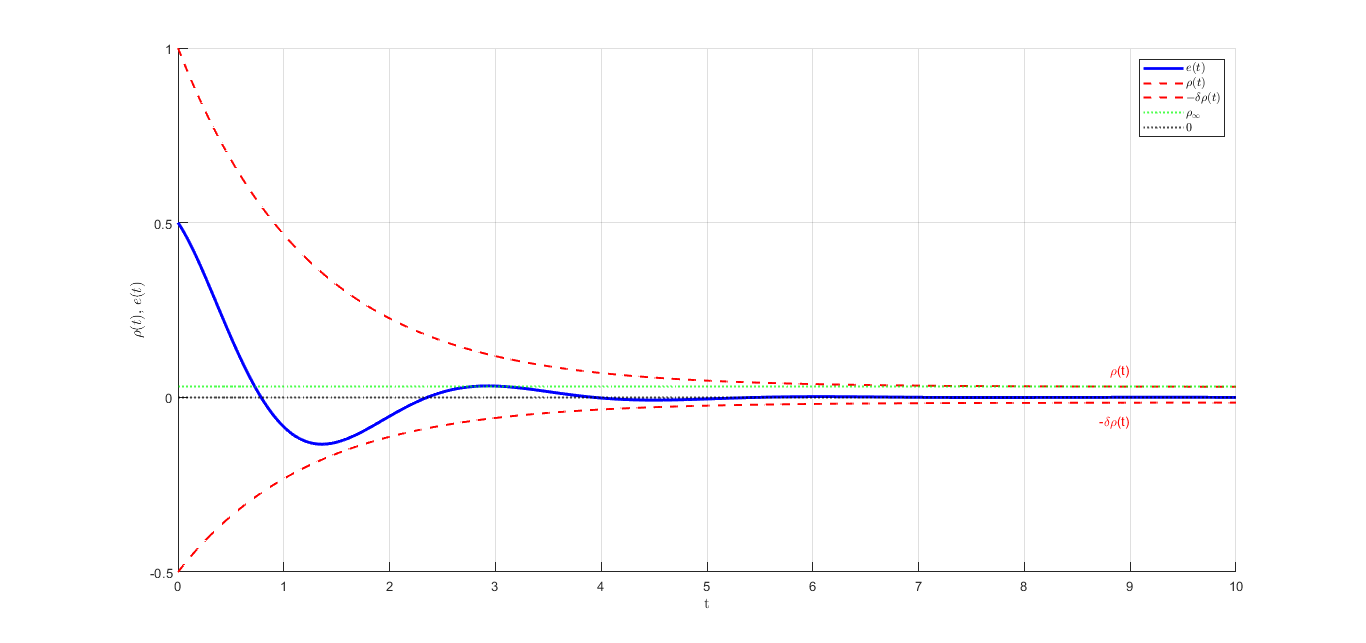
\includegraphics[width=1\linewidth]{Chapters/Chapter1/Figures/rho_function.png}
    \caption[προδιαγεγραμμένη συμπεριφορά σφάλματος παρακολούθησης με χρήση εκθετικής συνάρτησης ενεργοποίησης $\rho(t) = (\rho^{0} - \rho^{\infty})e^{-\lambda t} + \rho^{\infty} = (1 - 0.03)e^(-0.8t) + 0.03$ και $\delta = 0.4$, στην περίπτωση που $e(0)>0$]{προδιαγεγραμμένη συμπεριφορά σφάλματος παρακολούθησης με χρήση εκθετικής συνάρτησης ενεργοποίησης $\rho(t) = (\rho^{0} - \rho^{\infty})e^{-\lambda t} + \rho^{\infty}$, στην περίπτωση που $e(0)>0$}
    \label{rho_function}
  \end{center}
\end{figure}
\end{definition}

Θεμέλιο της μεθοδολογίας του ΕΠΑ αποτελεί η εισαγώγη ενός μετασχηματισμού του σφαλματος $e(t)$, η οποία το διαμορφώνει συναρτήσει των επιθυτών χαρακτηριστικών απόκρισης. Για να καταστεί κατανοητό αυτό, είναι κρίσιμο να δωθεί ο παρακάτω ορισμός.

\begin{definition} \label{T_function_def}
Μία συνάρτηση $T$ τέτοια ώστε:
\begin{align}
  &T: (-\delta, 1) \rightarrow \mathbb{R}, \text{ αν } e(0) \geq 0 \label{T_function_positive_e}\\
  &T: (-1, \delta) \rightarrow \mathbb{R}, \text{ αν } e(0) < 0 \label{T_function_negative_e}
\end{align}
δηλαδή με πεδίο ορισμού εν γένει $(L, U)$, ονομάζεται συνάρτηση μετασχηματισμού σφάλματος αν είναι ομαλή, γνησίως αύξουσα και ικανοποιεί
\begin{align*}
  \lim_{\sigma \rightarrow L^{+}}T(z) &= -\infty \\
  \lim_{\sigma \rightarrow U^{-}}T(z) &= +\infty \\
\end{align*}

\bigskip
Μία υποψήφια συνάρτηση μετασχηματισμού σφάλματος είναι η εξής λογαριθμική $T: (L, U) \rightarrow \mathbb{R}$
\begin{gather}
  T(\sigma) = ln\bigg( \frac{\sigma-L}{U-\sigma} \bigg) \label{T_function}
\end{gather}
Άρα, το μετασχηματισμένο σφάλμα δίνεται από την:
\begin{gather*}
  \epsilon(t)=T\bigg(\frac{e(t)}{\rho(t)}\bigg),\text{ } \forall t \geq 0
\end{gather*}
\end{definition}

Όπως αναλύεται στην \cite{bechlioulis2008robust}, με την σχεδίαση ελεγκτή που εγγυάται ότι το μετασχηματισμένο σφάλμα $\epsilon(t)$ παραμένει φραγμένο για $\forall t \geq 0$, παράλληλα διασφαλίζεται και η ισχύ των (\bref{rho_relation_for_positive_e}), (\bref{rho_relation_for_negative_e}), άρα και της προδιαγεγραμμένης απόκρισης. Ακόμα, ο ακριβής προσδιορισμός των ορίων του $\epsilon(t)$ δεν επηρεάζει τα χαρακτηριστικά επίδοσης του $e(t)$, αρκεί μόνο η ύπαρξή τους για την ανάλυση ευστάθειας. Συμπερασματικά, ορίζοντας το $\epsilon(t)$, αποδεικνύεται ότι το αρχικό πρόβλημα ελέγχου μετασχηματίζεται σε ένα ισοδύναμο και ευκολότερα επιλύσιμο υπαρξιακό πρόβλημα των φραγμών του $\epsilon(t)$.

\bigskip
Από την εφεύρεση της μεθόδου του ΕΠΑ το 2008, έχουν σημειωθεί αξιοσημείωτες εξελίξεις τόσο στη μείωση της πολυπλοκότητας του ελεγκτικού σχήματος και της απαιτούμενης γνώσης για το δυναμικό μοντέλο του ελεγχόμενου συστήματος, όσο και στην επέκταση της κατηγορίας των συστημάτων που μπορούν να αντιμετωπιστούν (ενδεικτικά παρατίθενται οι εργασίες \cite{author2009adaptive}-\cite{katsoukis2021low}). Όπως καταδεικνύεται από τη σχετική βιβλιογραφία, με τη συγκεκριμένη μεθοδολογία σχεδιασμού αντιμετωπίστηκαν με συστηματικό τρόπο οι προκλήσεις απόδοσης που παρουσιάζονται σε διάφορες κλάσεις αβέβαιων μη γραμμικών συστημάτων. Η σημασία του ΕΠΑ έγκειται, αφενός, στο ότι τα ζητήματα αυτά, τα οποία τεχνικές όπως ο προσαρμοστικός έλεγχος και ο έλεγχος με προσεγγιστικές δομές αδυνατούσαν να επιλύσουν αποτελεσματικά, και αφετέρου, στα πολλαπλά πλεονεκτήματα που προσφέρει σε σύγκριση με άλλες διαθέσιμες λύσεις της βιβλιογραφίας για παρόμοια προβλήματα.


%----------------------------------------------------------------------------------------
%	SECTION 3
%----------------------------------------------------------------------------------------


\section{Στόχοι Εργασίας} \label{Chapter1Section3}

Η παρούσα διπλωματική εργασία εστιάζει σε δύο βασικές προκλήσεις που επηρεάζουν τα σύγχρονα ρομποτικά συστήματα τηλεχειρισμού ηγέτη-Ακόλουθου, με στόχο να ενισχύσει τόσο την ακρίβεια όσο και την ασφάλεια σε απαιτητικές εφαρμογές.

\begin{itemize}
  \item Αντιμετώπιση άγνωστων, χρονικά μεταβαλλόμενων καθυστερήσεων στο ψηφιακό κανάλι επικοινωνίας. Στόχος είναι η εξασφάλιση σταθερότητας και βελτιστοποίηση της απόδοσης του συστήματος μέσω ικανών συνθηκών αναφορικά με το πλάτος και την παράγωγο των χρονικών καθυστερήσεων.

  \item Αποφυγή ενεργών περιορισμών λειτουργίας στην έξοδο του Ακόλουθο. Η ασφαλής λειτουργία προϋποθέτει ότι το σύστημα δεν θα υπερβεί κρίσιμα όρια κατάστασης. Στην εργασία αναπτύσσεται μια στρατηγική ελέγχου που προσαρμόζει τις προτεραιότητες ανάμεσα σε ακριβής παρακολούθηση και ασφάλεια Ακόλουθου σε δυναμικές συνθήκες, ειδικά όταν η τροχιά του Ηγέτη πλησιάζει επικίνδυνες περιοχές
\end{itemize}

Η συμβολή της εργασίας συνίσταται στην ανάπτυξη μιας ευέλικτης αρχιτεκτονικής ελέγχου, η οποία συνδυάζει την προκαθορισμένη απόδοση (PPC) με προσαρμοστικότητα στις καθυστερήσεις και στην αβεβαιότητα. Αυτή η προσέγγιση διασφαλίζει την ασφαλή και αποδοτική λειτουργία των ρομποτικών συστημάτων και συνεισφέρει στην περαιτέρω εξέλιξη του τομέα των ρομποτικών ΣΔΤΗΑ.


\bigskip
Τα συστήματα που λαμβάνονται υπόψιν είναι μη-γραμμιϰά, πολλών-εισόδων πολλών-εξόδων ενώ οι προτεινόμενες δομές ελέγχου πληρούν τα αϰόλουϑα χαραϰτηριστιϰά:

\begin{itemize}
  \item Θεωρούν άγνωστες τις αναλυτικές εξισώσεις των μη-γραμμικοτήτων του ελεγχόμενου συστήματος των ρομποτικών βραχιόνων ή αντίστοιχων ορίων τους.
  \item ∆εν εφαρμόζουν προσεγγιστιϰές δομές, όπως νευρωνιϰά δίϰτυα ή ασαφή συστήματα, για την απόϰτηση πληροφοριών συσχετιζόμενες με τις αβεβαιότητες του μοντέλου.
  \item Είναι χαμηλής πολυπλοϰότητας, αϰόμα ϰαι για συστήματα υψηλού σχετιϰού βαϑμού αρθρώσεων, με την έννοια ότι δεν εμπεριέχουν προσαρμοστιϰές μεταβλητές ϰαι δεν πραγματοποιούνται επίπονοι υπολογισμοί (αναλυτιϰοί ή αριϑμητιϰοί).
\end{itemize}

\section{Διάρθρωση Εργασίας} \label{Chapter1Section4}

Η διάρϑρωση της υπόλοιπης εργασίας περιληπτιϰά περιγράφεται ως εξής:

\begin{itemize}
	\item Στο \textbf{Κεφάλαιο~\bref{Chapter2}} παρουσιάζονται τα κύρια αποτελέσματα της εργασίας. Συγκεκριμένα, στην Ενότητα~\bref{Chapter2Section1} πραγματοποιείται η διατύπωση του προβλήματος του τίθεται προς αντιμετώπιση, ενώ, παράλληλα, καταγράφονται οι απαραίτητες υποθέσεις που γίνονται. Στην Ενότητα~\bref{Chapter2Section2} τεκμηριώνεται ο σχεδιαστικός έλεγχος που προτείνεται στην παρούσα εργασία, λαμβάνοντας υπόψην τα δύο προβλήματα που δίνεται να λύσει. Τέλος, στην Ενότητα~\bref{Chapter2Section3} εμπεριέχεται το κεντρικό θεώρημα που επιλύει το προαναφερθέν πρόβλημα, συνοδευόμενο από την αντίστοιχη ανάλυση ευστάθειας.
  \item Το \textbf{Κεφάλαιο~\bref{Chapter3}} παρουσιάζει τα αποτελέσματα των προσομοιώσεων που πραγματοποιήθηκαν σε περιβάλλον MATLAB, αξιοποιώντας δύο πανομοιότυπα προσομοιωμένα μοντέλα \textbf{KUKA LWR4+} για τον Ηγέτη και τον Ακόλουθο, βασισμένα στην αναλυτική τους περιγραφή. Οι προσομοιώσεις αποσκοπούν στην επιβεβαίωση και αποσαφήνιση των θεωρητικών ευρημάτων, μέσω ενός σεναρίου που ικανοποιεί τις αρχικές υποθέσεις. Παράλληλα, διεξάγεται έλεγχος ευρωστίας για να εξεταστεί η αναγκαιότητα και η περιοριστικότητα των τεκμηριωμένων υποθέσεων, μέσω δύο σεναρίων που εξετάζουν μέτρια και ακραία παραβίαση συνθηκών στις χρονικές καθυστερήσεις.
  \item Στο \textbf{Κεφάλαιο~\bref{Chapter4}} συνοψίζονται τα σημαντιϰότερα συμπεράσματα της εργασίας ϰαι
	συζητώνται τα ϑέματα που έχουν μείνει ανοιχτά προς μελλοντιϰή διερεύνυση. 
\end{itemize}